%\documentclass[paper]{geophysics}
\documentclass[manuscript,revised]{geophysics}

% An example of defining macros
\newcommand{\rs}[1]{\mathstrut\mbox{\scriptsize\rm #1}}
\newcommand{\rr}[1]{\mbox{\rm #1}}

\newcommand{\psm}{\textit{PSM} }
\newcommand{\twod}{two-dimensional }
\newcommand{\thrd}{three-dimensional }

\begin{document}

\title{tmp title: MUSC source}

\renewcommand{\thefootnote}{\fnsymbol{footnote}} 

\ms{GEO-Example} % manuscript number

\address{
\footnotemark[1]LUNAM-IFSTTAR, \\
\footnotemark[2]OSUNA \\
\footnotemark[1]LPGN, \\}
\author{Damien Pageot\footnotemark[1]\footnotemark[2], Donatienne Leparoux\footnotemark[1], Mathieu Le Feuvre\footnotemark[1], Olivier Durand\footnotemark[1] and Yann Capdeville\footnotemark[3]}

\footer{Example}
\lefthead{Dellinger \& Fomel}
\righthead{\emph{Geophysics} example}

\maketitle

\begin{abstract}
\end{abstract}

% ## INTRODUCTION
\section{Introduction}

% #### Nature and scope of the problem
\noindent Since decades, geophysicists develop numerical inversion and imaging methods for seismic measurements (receiver function analysis  \citep{Ammon_1991_IRE}, ray-based methods \citep{Jones_PRM_2013}, finite-frequency tomography \citep{Montelli_FFT_2004}, inversion-based methods \citep{Virieux_FWI_2009}) to determine the structures and the physical properties of the Earth at several scales as subsurface (civil engineering), crustal, regional or global. These methods, like Full Waveform Inversion (FWI), are still in development and are mostly validated using synthetic data which are generally computed using the same wave propagation modeling engine used in the inverse problem process. In other terms, the synthetic data are computed with some assumptions (for example acoustic approximation or \twod) which are the same in the inverse problem. Although, this \textit{inverse crime} \citep{Wirgin_TIC_2004} is particularly useful to validate an algorithm in its early development stage, it does not allow to assess the efficiency of the method for real seismic data. Moreover, because no one known precisely the Earth interior, it is difficult to evaluate the capacity of a method to recover physical parameters and structures from real seismic data which can lead sometimes to geological interpretation of numerical artifacts \citep{Morozov_ARF_2004}. Thus, it is necessary to add a step for which imaging methods will be tested for experimental seismic measurements obtained under controlled conditions.      

\noindent The best way to satisfy this need is to use Physical Small Scale Modeling Methods (noted \psm subsequently). \psm were used since several years to study the propagation of waves in various media with several stage of complexity, from acoustic wave propagation in homogeneous media to elastic wave propagation in \thrd heterogeneous anisotropic media \citep{Rieber_EWP_1936,Howes_SMS_1953,Hilterman_TDM_1970,French_MRP_1974,Bishop_LVM_1985,Pratt_FWI_1999,Favretto_NMT_2013,Sarkar_TPM_2003,Isaac_SMS_1999}, and allow to generate experimental seismic data under well-controlled conditions. Some methods exist to produce this kind of data for different purpose \citep{Wong_SPM_2009} and the MUSC Laboratory \citep{Bretaudeau_SSA_2008b,Bretaudeau_SSM_2011,Bretaudeau_FWI_2013}, \textit{Mesure Ultrasonore Sans Contact} in French, in one of them. MUSC is designed to allow (1) wide-angle on-shore acquisitions modeling both body waves and surface waves, (2) automatic multisource-multireceiver measurements with a high-productivity, (3) high-precision source-receiver positioning and (4) high-precision recording of absolute surface displacement without coupling effects. 

% #### State the objectives
\noindent Our objective here is to increase the potential of the MUSC system as a reliable tool for generating experimental data which will be distributed in the scientific community. 
\noindent Thus we present two studies of experimental data in order to : 1) refine the comparison between numerical and experimental data by taking into account the 2D/3D effects through an alternative way and 2) identify the reproducibility of the source impact. These approaches complete the knowledge of the system and facilitate the achievement of massive multi-source and multi-receiver data simulating subsurface seismic experimental campaigns.

% #### Describe the method of investigation
\noindent To achieve these objectives, we used a seismic wave modeling code based on the Spectral Element Method \citep{Komatitsch_SEM_1998,Komatitsch_ISM_1999,Komatitsch_SEM_2005,Festa_PML_2005}. This method has several advantages compared to finite differences and finite elements, such as: (1) a weak formulation which can naturally take into account the free surface, (2) an explicit scheme in time facilitating parallelization and reducing the computational cost, (3) a spatial discretization (mesh) convenient for the representation of complex environments and (4) high precision results and low numerical dispersion.

% #### Describe the principal results of the investigation

\noindent Thus, this article is organized as follow. In a first part, we present he MUSC laboratory and the SEM code used for the studies. In a second part, we present two coupled studies of experimental data in order to: (1) refine the comparison between numerical and experimental data by taking into account the geometrical spreading effects between \twod and \thrd data through an alternative way, and (2) identify the reproducibility of the source impact to [...].


% ## METHODS
\section{Methods}

% #### MUSC bench
\subsection{Physical modeling: MUSC Bench}

\noindent The MUSC bench \citep{Bretaudeau_SSA_2008b,Bretaudeau_SSM_2011,Bretaudeau_FWI_2013} is built to experimentally reproduce field seismic data with a great accuracy on small scale model. Figure \ref{panel_musc_bench} shows the bench and its components. MUSC is composed of a honeycomb tab and two arms which control the source and the receiver position with a precision of 10 $\mathrm{\mu m}$.

\noindent The receiving system of MUSC Laboratory is composed of a laser interferometer. The principle of this laser is based on a phase shift of the reflected laser signal due to the wave propagation in the material. A real-time calibration value enables a continuous conversion to a nanometric displacement. The focal diameter of the laser on the model surface is about several micrometers and allows a detection limit of $\mathrm{2.5\ nm}$ in the frequency range from 30 kHz to 20 MHz.

\noindent The seismic source is simulated by a piezoelectric transducer relied to a launching and synchronization system. This system provides more energy than a laser impulse source \citep{Bretaudeau_PHD_2010,Bretaudeau_SSM_2011} and allows to choose the source in terms of waveform, \textit{i.e.}, Gauss source, Ricker source, central frequency $f_{0}$ and time delay $t_{0}$. The source is generated by a waveform generator and is then amplified before transmitted to the small-scale-model. In the framework of seismic physical modeling, the source must be as closed as possible to a normal point source. Thus, the piezoelectric source is coupled with an adapter in order to reproduce the spatial energy repartition (limiting directivity) and conserving the waveform as shown in figure \ref{piezo-source-validation}.

\noindent For the purpose of small scale modeling, the change of scale must keep the relationship between observables. For most of seismic imaging methods, the significant physical parameters are the compressional and shear waves velocities, $V_{P}$ and $V_{S}$ respectively, the density $\rho$ and the quality factor $Q$. When scaling the model, many parameters can be modified: the distances, the time scale, the amplitudes of the signals, the viscoelastic properties, etc. Hence, the predominant factor is the wavelength $\lambda = V / f$, where $V$ is the wave velocity and $f$ the frequency. Thus, physical and mechanical parameters are modified to preserve the ratio $\lambda_{real} = \xi \lambda_{scale}$ where $\xi$ is the scale ratio. It is therefore necessary to act directly on the time-frequency scales. Assuming the materials used to build the small scale model have the same mechanical properties ($V_{P}$, $V_{S}$, $\rho$) than the natural media, it is straightforward to obtain the scale ratios for parameters involved in seismic experiment.

\noindent For near surface experiments, the scale ratio $\xi$ is about $1000$ which means that the central frequency $f_{0}$ of the source is few $kHz$ (generally 100 kHz but can be more or less), distances are in $mm$ (acquisition length around 50 mm typically) and time unit is $ms$.

\noindent Small-scale models are generally made of metal, thermoplastic or melted epoxy resin-based materials \citep{Bretaudeau_FWI_2013,Bretaudeau_SSM_2011,Bretaudeau_SSA_2008b}. These materials allow to reproduce complex geometries and have a large panel of physical and mechanical properties. These materials have the advantages to have physical properties closed to natural soil materials. The models are generally over-sized to easily separate reflected waves on boundaries from the rest of the signal. 

% #### Spectral Element Method
\subsection{Numerical modeling: Spectral Element Method}

\noindent Various numerical methods exist to resolve the equation of motion in arbitrary elastic media. The most widely used is the Finite-Differences (FD) method \citep{Virieux_PSV_1986,Levander_PSV_1988,Robertsson_FDM_1994,Pratt_EWM_1990,Stekl_VEM_1998,Saenger_FDM_2004} which estimates each derivative on a regular Cartesian grid using a Taylor development \citep{Moczo_FDM_2004} of order \textit{n}. FD is simple to implement but quickly shows some limitations: the Cartesian grid is defined by the minimum propagated wavelength ($\lambda_{min}$) in the full media and is unable to reproduce properly complex topography and interfaces. Moreover, \citet{Saenger_FDM_2000} show that 60 points by wavelength ($\lambda$) are needed to model propagation of Rayleigh wave in order $n=2$ where only 15 points by $\lambda$ are required to model propagation of body waves which increases drastically the numerical cost in case of near-surface modeling experiment. The Finite-Elements Method (FEM) is another popular method used for wave propagation modeling \citep{Lysmer_FEM_1972,Seron_FEM_1990,Hulbert_FEM_1990}. FEM is based on a variational formulation of the equation of motion and gives a continuous approximate solution in space using polynomial basis functions defined on each node of each cell of the mesh. The natural boundary conditions of FEM is the free surface and the triangular (in 2D) or tetraedric (in 3D) unstructured meshes are well adapted to complex media and topography. However, low polynomial basis are inadequate with fine spatial discretization and the required discretization to obtain precise and non-dispersive solution in numerically costly. 

\noindent Recently, the Spectral Element Method (SEM), used in fluid dynamics, was adapted to seismic wave propagation. 

\noindent The SEM is based upon a high-order piecewise polynomial approximation of the weak formulation of the wave equation. It combines the accuracy of the pseudo-spectral method with the flexibility of the finite-element method \citep{Tromp_SEM_2008}. 

\noindent In this method, the wave-field is represented in terms of high-degree Lagrange interpolants, and integrals are computed based upon Gauss-Lobatto-Legendre (gll) quadrature. This combination leading to a perfectly diagonal mass matrix leads in turn to a fully explicit time scheme which lends itself very well to numerical simulations on parallel computers. It is particularly well suited to handling complex geometries and interface matching conditions \citep{Cristini_SEM_2012}. 

\noindent As in FEM, all boundary of the domain are reflecting and the free surface is the natural condition.  In order to simulate infinite or semi-infinite domain, SEM uses Perfect Match Layers boundary conditions \citep{Berenger_PML_1994,Festa_PML_2005} but are not used here.
 
\noindent The typical element size that is required to generate an accurate mesh is of the order of $\lambda$, $\lambda$ being the smallest wavelength of waves traveling in the model.

\noindent Models are meshed in 2D with quadrangles using the open-source software package GMSH \citep{Geuzaine_MSH_2009}. 

% ## Results
\section{Results}

% #### From point-source to line-source acquisition
\subsection{From point-source to line-source acquisition}

\noindent In the framework of wave propagation modeling and waveform inversion, most of available algorithms are limited to the \twod approximation especially for computational cost causes. Thus, line-source seismograms are required as observed data to be compared to synthetic seismograms or for inversion processes.

\noindent However, MUSC is designed to produce \thrd experimental seismograms from a piezoelectric source selected to be as closed as possible to a point source. Generally, the correction of the geometrical spreading is done by convolving each trace by $\mathrm{\sqrt{t^{-1}}}$, where $t$ is the travel-time, with or without offset conditioning. The correct phase can then be obtained using a source wavelet estimation method \citep{Bretaudeau_SSM_2011}.

\noindent Recently, \citet{Forbriger_LSS_2014} and \citet{Schafer_LSS_2014} have developed, and successfully applied to synthetic seismograms, an hybrid method to convert the \thrd geometrical spreading in \twod spreading using both convolution tapering and offset dependent scaling of the waveform. However, these pre-processing methods are not perfect and can not ne easily automated and the results are strongly conditioned by user's experience and attempts.

\noindent Here, we take advantage of the experimental framework to explore an alternative approach specific to MUSC. Contrary to field experiments, it is possible to generate a pseudo-line-source finely sampled by multiple point-sources, perpendicular to the acquisition line. 

\noindent Each point-source must be enough close each other so the resulting source being a line-source in the sense of Huygens principle. To do that, we consider that the length of the line must be equal, at least, $L \geq 4\lambda_{max}$ and the sampling interval $ds \leq 10 / \lambda_{min}$. Given the material's properties, we choose $L=240\ mm$ and $ds=0.5\ mm$ which leads to 481 point-source locations. The line of point-source is located at ?? mm distance. Four receiver positions have been selected: 90, 95, 100 and 105 mm offset from the source. The source wavelet is a Ricker with a central frequency $f_{0}=100\ kHz$.Each receiver is perpendicular to and centered on the line-source. For each receiver position, the complete signal is stack along source position to obtain an equivalent \twod line-source response.
 
\noindent To evaluate the efficiency of the method, experimental line-source responses will be compared to point-source and equivalent line-source responses using the cross-correlation coefficient (\textbf{cc}) and the root mean square (\textbf{rms}) ratio. These values are presented in table \ref{cc-rms}. \textbf{cc}$_init$ and \textbf{rms}$_init$ correspond to direct evaluation whereas \textbf{cc}$_final$ corresponds to the best \textbf{cc} obtained and \textbf{rms}$_final$ is the corresponding \textbf{rms}.

\noindent Figures \ref{panel_amplitude}(a,b,c,d) show the comparison between experimental traces obtained using a point-source and a line-source for source-receiver offsets 90, 95, 100 and 105 mm respectively. It is straightforward that these waveforms are not similar in terms of both phases (\textbf{cc}$<$0.2) and amplitude (\textbf{rms}$>$1.2). Even after dephasing point-source response to the line-response in term of phase (\textbf{cc}$>$0.6), amplitudes do not match (\textbf{rms}$>$0.6). These results confirm that using raw point-source responses in a \twod inversion process or imaging method can be critical in terms of convergence and validity of the results since these methods are built over phase and/or amplitude similarity.
%Even if waveforms seem quite similar, amplitude differences and phase shifts between point-source and line-source responses may be critical in a \twod FWI process as shown by \citet{Schafer_LSS_2014}.

\noindent Figures \ref{panel_amplitude}(e,f,g,h) show the comparison between experimental traces using a line-source and a point-source after geometrical spreading corrections (equivalent line-source response) for the same previous source-receiver offsets. The cross-correlation coefficient \textbf{cc} for these waveforms are greater than 0.69 but with \textbf{rms} greater than 0.66 and between 0.48 and 0.54 after phase fitting (\textbf{cc}$>$0.85). These results denote that the experimental line-source response is correct in terms of phase compared to an equivalent line-source response. However, \textbf{rms} are still great even if they are smaller than previously. This can be explained by small differences in terms of waveforms and phases which are critical in the final \textbf{rms} results. Moreover, the \textit{hybrid} method to obtain the equivalent line-source response from a point-source response needs accurate parametrization to obtain the best result which is not necessarily in a good agreement with the attempt true line-source response.   

\noindent These results show that the line-source emulation on the MUSC laboratory is efficient and can produce data suitable for imaging methods such as 2D FWI.


% #### Experimental source reproducibility
\subsection{Experimental source reproducibility}

\noindent To assess the ability of MUSC to provide reproducible data, \textit{i.e.} to evaluate the reproducibility of the source impact, several physical modeling were performed on a homogeneous epoxy-resin block for which the seismic waves velocities and the intrinsic attenuation are known : $\mathrm{V_{P}=2300\ m.s^{-1}}$, $\mathrm{V_{S}=1030\ m.s^{-1}}$, $\mathrm{\rho=1300\ kg.m^{-3}}$ and $\mathrm{Q=30}$. 

\noindent Six realizations have been acquired on this model with a similar geometry setup, i.e. 121 receivers positions with an increment equal to 1 mm and a minimum offset of 10 mm. The numerical wavelet sent to the piezoelectric transducer source is a Ricker signal with a central frequency of 100 kHz. However, the source waveform is modified by the physical coupling effect of the transducer. 

\noindent First, source wavelet were estimated for each experiment (Figure \ref{panel_srcest_2d}(a)) using a linear source wavelet estimation method based on a stabilized deconvolution \citep{Pratt_FWI_1999}. The effective sources show different oscillations after the main pulse, due to internal echoes in the transducer. These secondary oscillations have a very similar shape from an experiment to another, as well as the global signal shape even if some small differences of amplitudes appear for the main pulse. Figure \ref{panel_srcest_2d}(b,c,d,e,f,g) show numerically propagated signals after convolution with estimated source wavelets for the offset of 60 mm. The corrected numerical seismograms are in good agreement with the experimental seismograms. The value of the correlation coefficient ($> 0.98$, also presented in the figure) confirms the great efficiency of the wavelet source assessment process.

\noindent In a second step, a unique source wavelet is estimated by taking into account the 6 experiments together (figure \ref{panel_srcest_2d_mean}(a)). The resulting source parameters were applied to the synthetic signals (figure \ref{panel_srcest_2d_mean}(b,c,d,e,f,g)) for the same receiver position as previously. As in the previous case, the corrected seismograms are in good agreement with the experimental seismograms (correlation coefficients $\mathrm{>}$ 0.96).  

\noindent These last results, based on an average estimated source wavelet show that the effective impulse source emitted by the transducer in the MUSC measurement bench is stable enough to ensure a robust reproducibility of the source. Therefore, concerning the key issue of the source knowledge, experimental data acquired in the MUSC laboratory can be efficiently processed by imaging methods like Full Waveform Inversion (FWI) with only one estimation step for all the multi-source and multi-receivers data.

% ## CONCLUSIONS

\section{Conclusions}

\noindent These two studies allow to refine the capacity of the physical modeling designed for seismic experiments simulation by 1) completing the validation of the measurement through comparison of numerical and experimental data generated by a realistic 2D source line and 2) assessing the reproductivity of the effective source emitted in a model. These improvements allow to provide and distribute experimental reduced scale data to the scientific community as benchmark datasets.

% ## PLOTS
\section{Plots}

\subsection*{Equations}

\subsection*{Figures}

% #### Fig:: panel_musc_bench
\begin{figure}[!h]
	\centering
	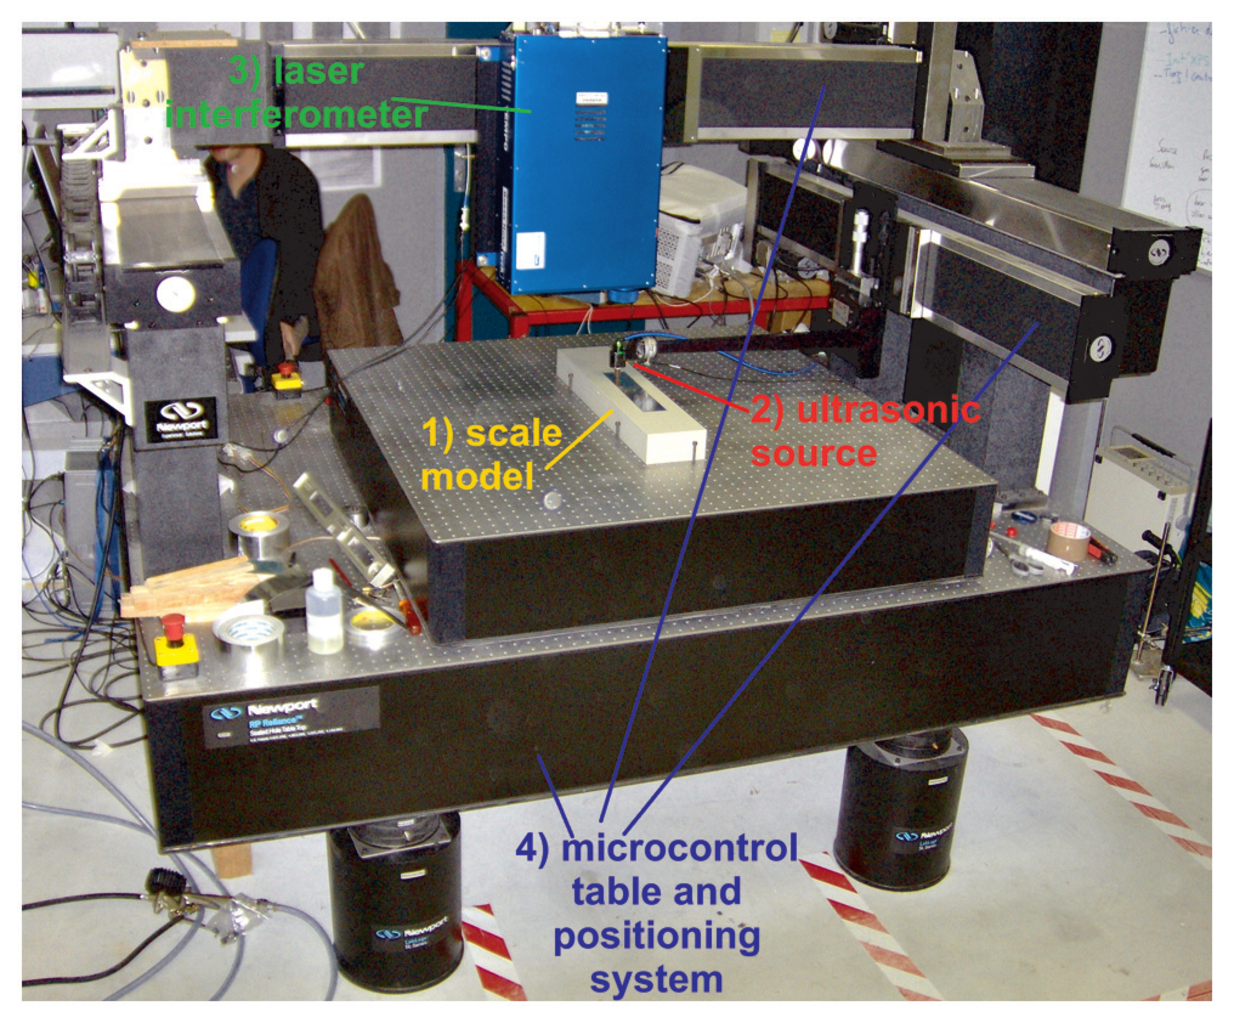
\includegraphics[scale=0.4]{fig/panel_musc_bench.eps}
	\caption{Photograph of the MUSC ultrasonic laboratory (from \citet{Bretaudeau_FWI_2013} )with its four components: (1) a small-scale model of the underground, (2) an optical table with two automated arms moving above the model, (3) a laser interferometer recording ultrasonic wave propagation	at the model surface, and (4) a piezoelectric ultrasonic source generating ultrasonic waves in the model.}
	\label{panel_musc_bench}
\end{figure}

% #### Fig:: panl_multisrcrec
\begin{figure}[!h]
	\centering
	\includegraphics[scale=0.4]{fig/panel_multisrcrec.eps}
	\caption{Example of multi-source multi-receiver record on the MUSC bench for a two-layer model (bialt).}
	\label{panel_multisrcrec}
\end{figure}

% #### Fig:: piezo-source-validation
\begin{figure}[!ht]
	\centering
	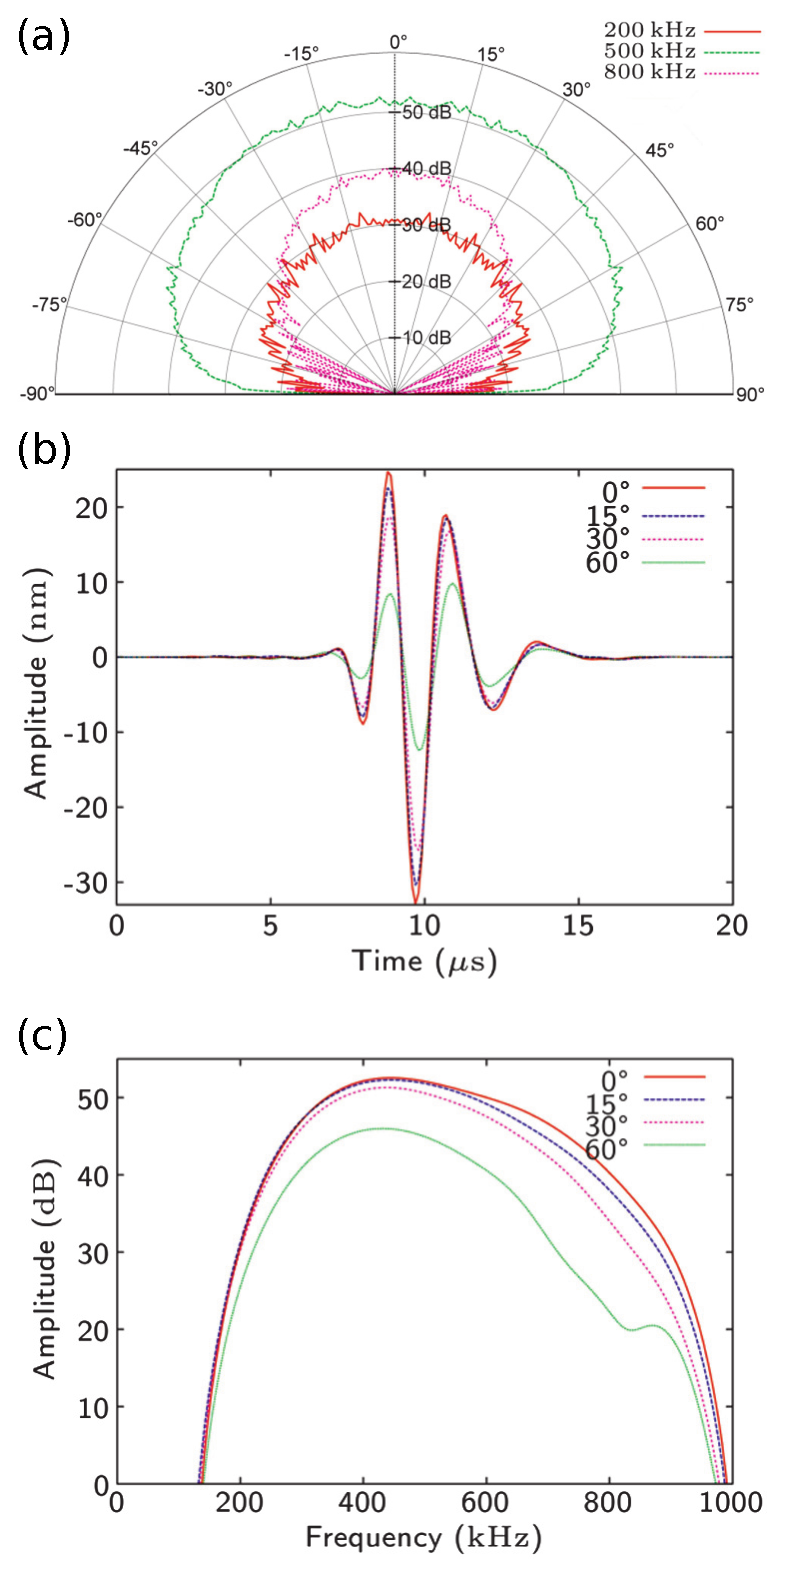
\includegraphics[scale=0.4]{fig/piezo-source-validation.eps}
	\caption{Validation of the piezoelectric source coupled with an adapter \citep{Bretaudeau_SSM_2011}. (a) Directivity diagrams (dB) for the high-frequency source Panametrics\textregistered with conical polyurethane adapter: three frequencies — normal particle displacement. (b) Temporal signals and (c) amplitude spectrums for the high-frequency source Panametrics\textregistered with a conical polyurethane adapter in transmission through a PVC cylinder for	various angles of incidence: O, 15, 30, and 60 degrees — normal particle displacement.}
	\label{piezo-source-validation}
\end{figure}

% #### Fig:: panel_bialt_model
\begin{figure}[!h]
	\centering
	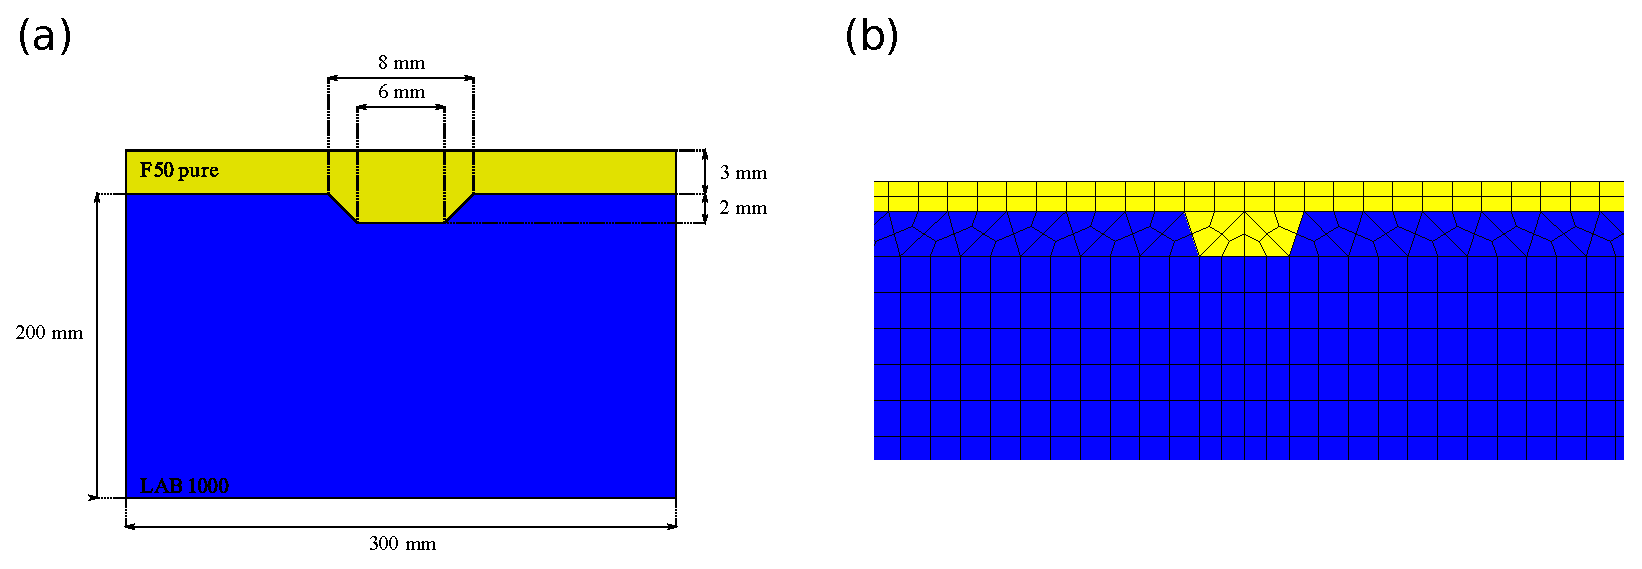
\includegraphics[scale=0.4]{fig/panel_bialt_model.eps}
	\caption{(a) Schematic representation of the so-called \textit{BiAlt} model. (b) Zoom in the two-dimensional mesh designed for the numerical version of the \textit{BiAlt} model.}
	\label{panel_bialt_model}
\end{figure}

% #### Fig:: panel_bialt_2d3d
\begin{figure}[!h]
	\centering
	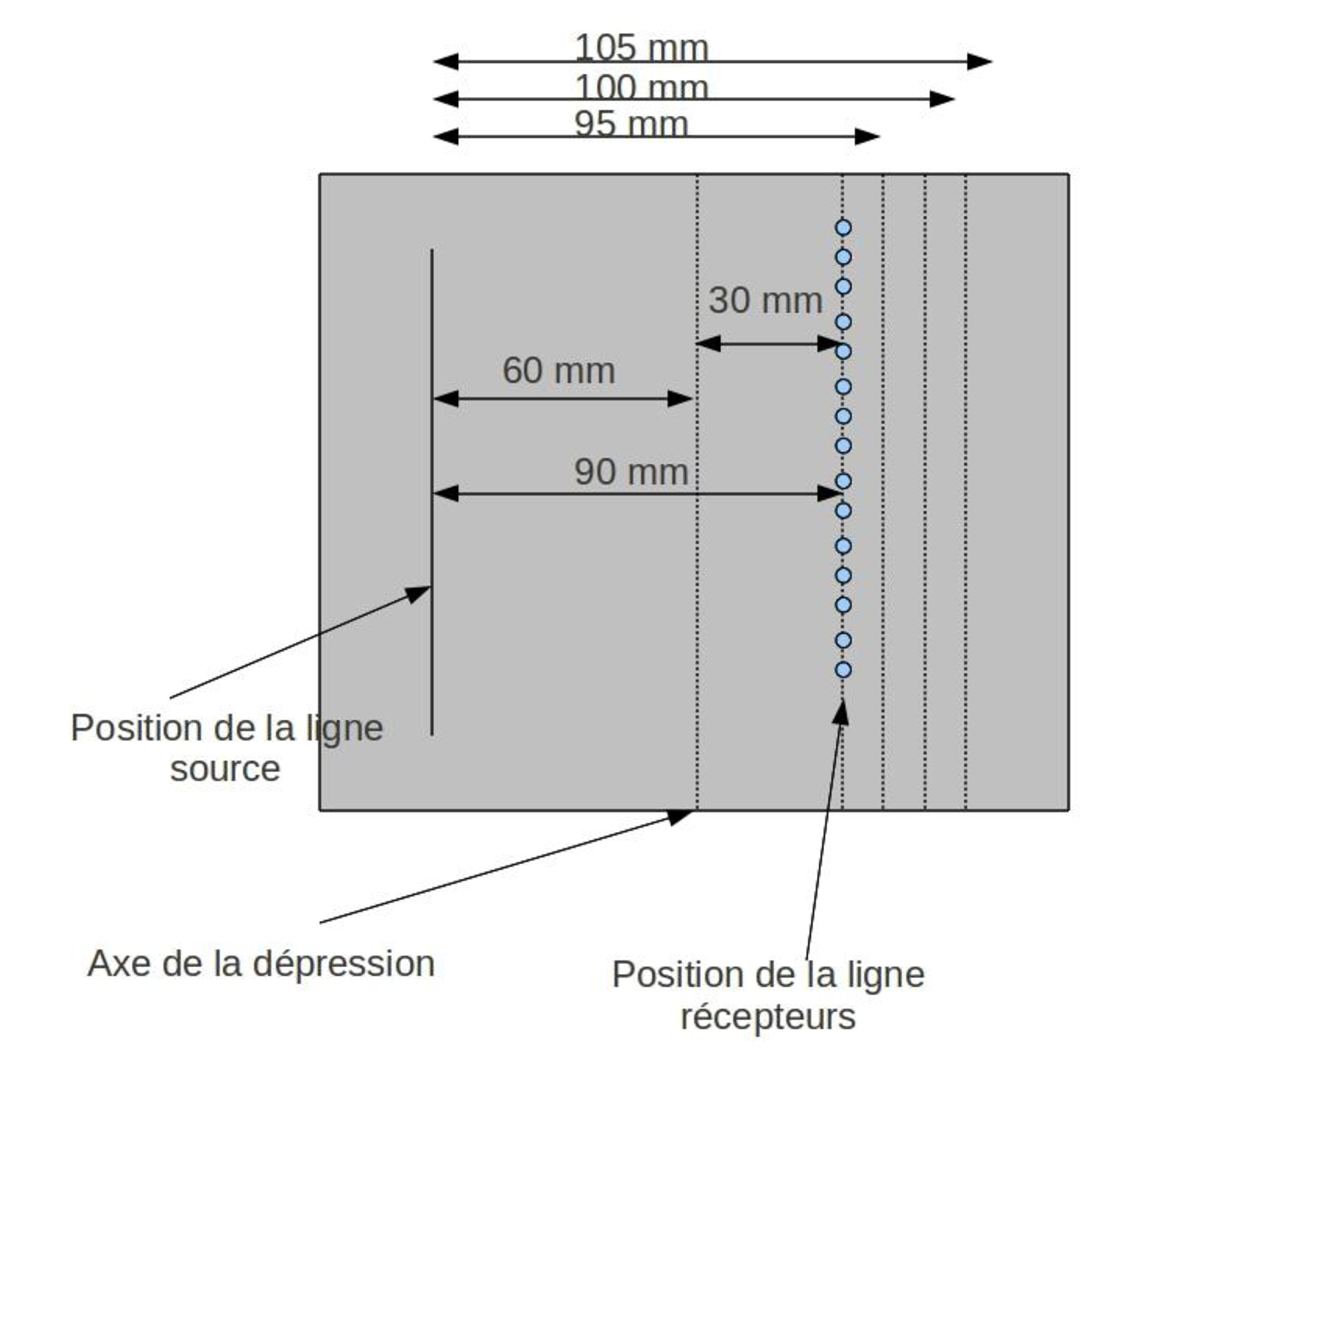
\includegraphics[scale=0.4]{fig/amplitude_acqui_principle.eps}
	\caption{.}
	\label{amplitude_acqui_principle}
\end{figure}

\begin{figure}[!h]
	\centering
	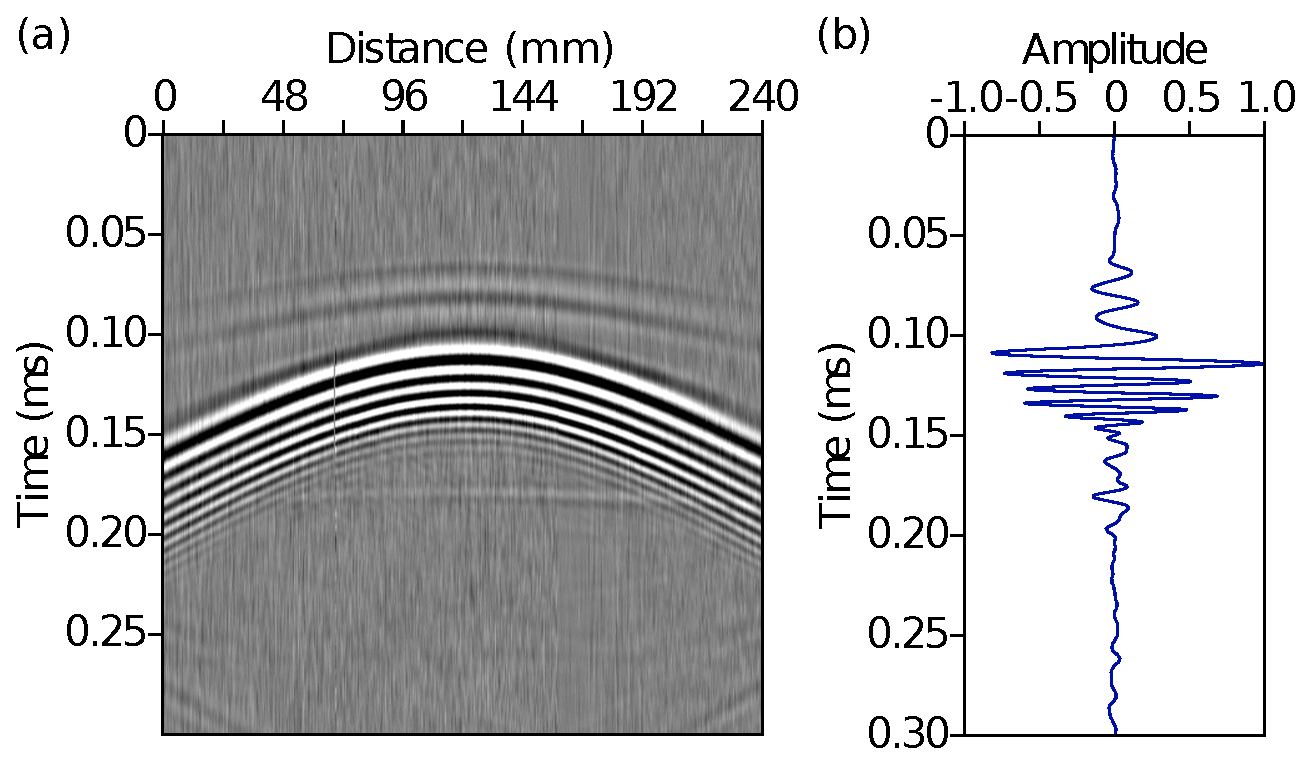
\includegraphics[scale=0.4]{fig/amplitude_stack_principle.eps}
	\caption{.}
	\label{amplitude_stack_principle}
\end{figure}

\begin{figure}[!h]
	\centering
	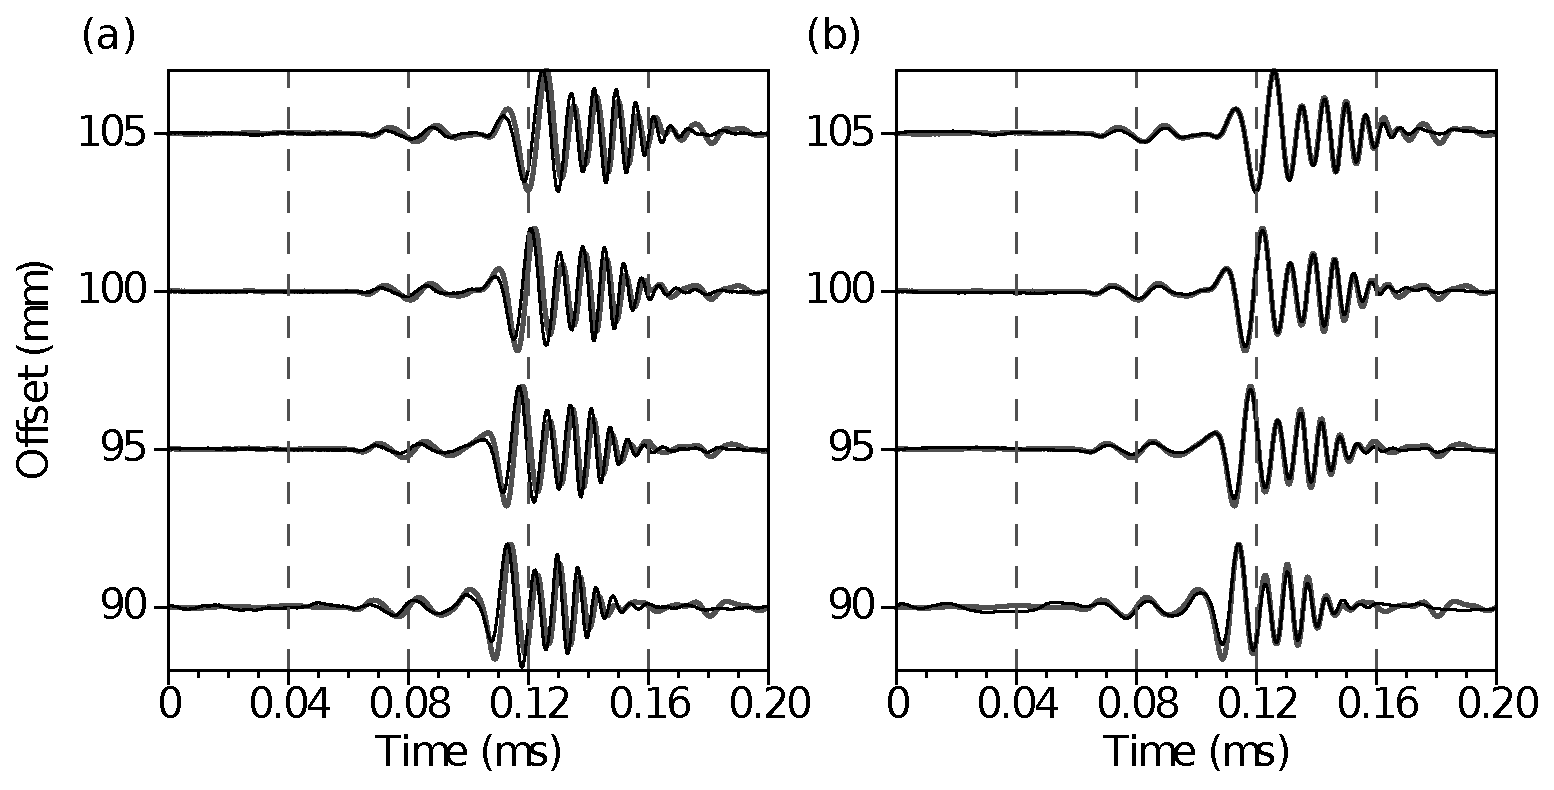
\includegraphics[scale=0.5]{fig/bialt_2d3d_merge.eps}
	\caption{(a) Comparison between an experimental seismogram for a point-source (black), an experimental seismogram for a line-source (grey) for 90, 95, 100 and 105 mm offset respectively. (b) Comparison between an experimental seismogram for a line-source (grey), and for a point-source corrected from geometrical spreading (black) for 90, 95, 100 and 105 mm offset respectively \textbf{cc} gives the correlation factor between line-source and point-source responses.}
	\label{panel_amplitude}
\end{figure}

% #### Fig:: panel_srcest_2d
\begin{figure}[!h]
	\centering
	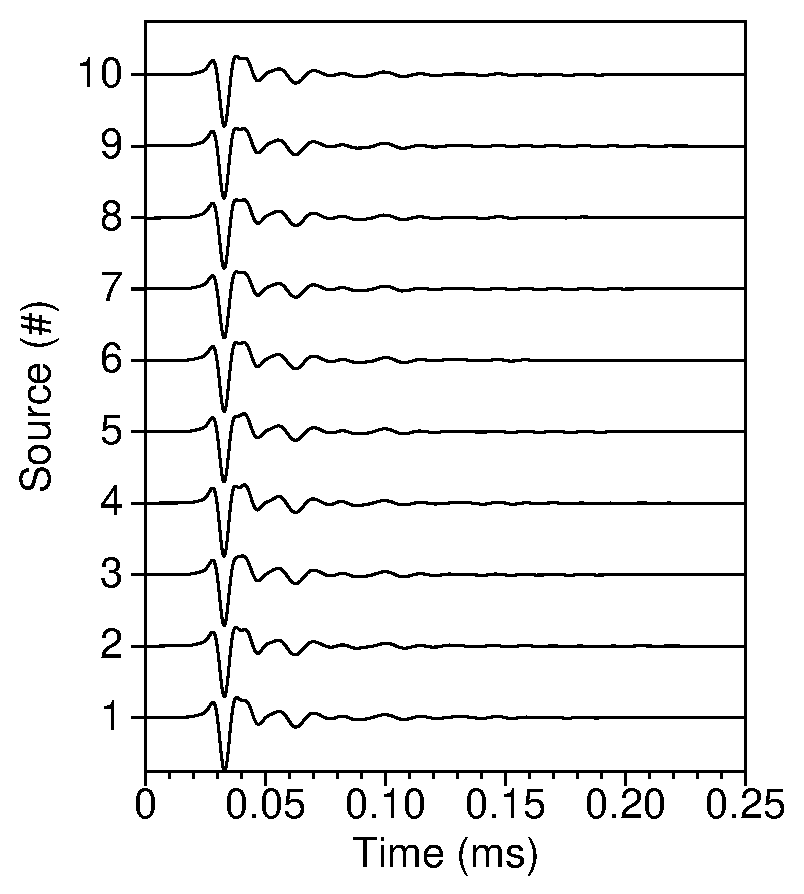
\includegraphics[scale=1.0]{fig/F50_once_srcest_wig.eps}
	\caption{(a) Comparison between six estimated source wavelets (\textit{ESW}) calculated for each experiment. (b,c,d,e,f,g) Comparison between experimental traces (black) and numerically simulated traces corrected with the corresponding estimated effective source (colored). \textbf{r} gives the correlation factor between numerical simulation from the estimated effective source and experimental traces.}
	\label{panel_srcest_2d}
\end{figure}

\begin{figure}[!h]
	\centering
	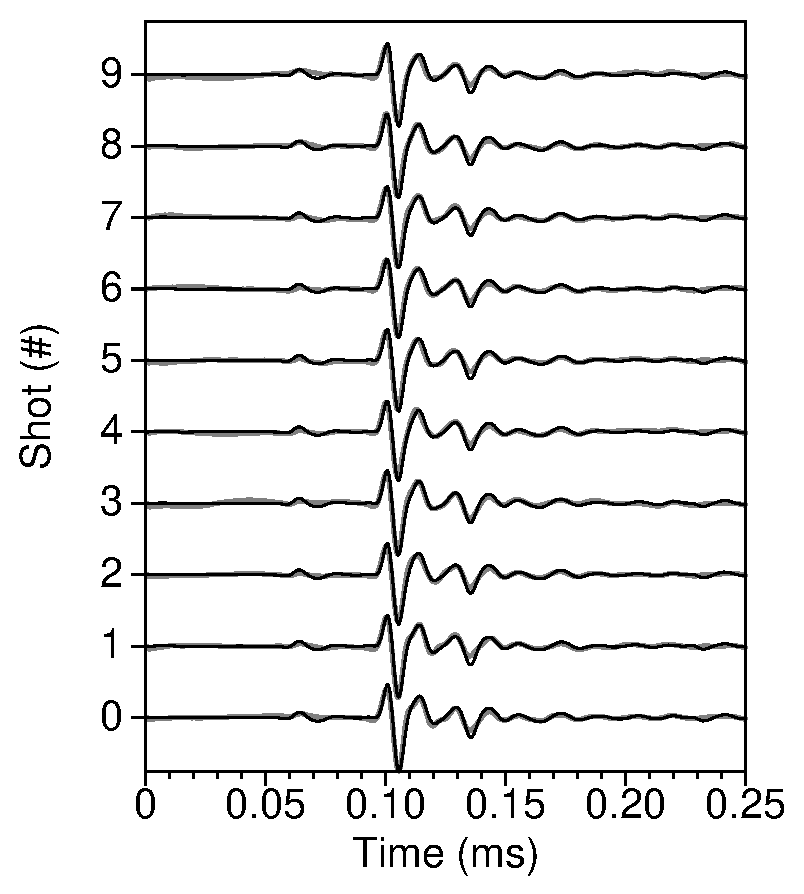
\includegraphics[scale=1.0]{fig/F50_CT_once.eps}
	\caption{.}
	\label{panel_srcest_2d_comp}
\end{figure}

% #### Fig:: panel_srcest_2d_mean
\begin{figure}[!h]
	\centering
	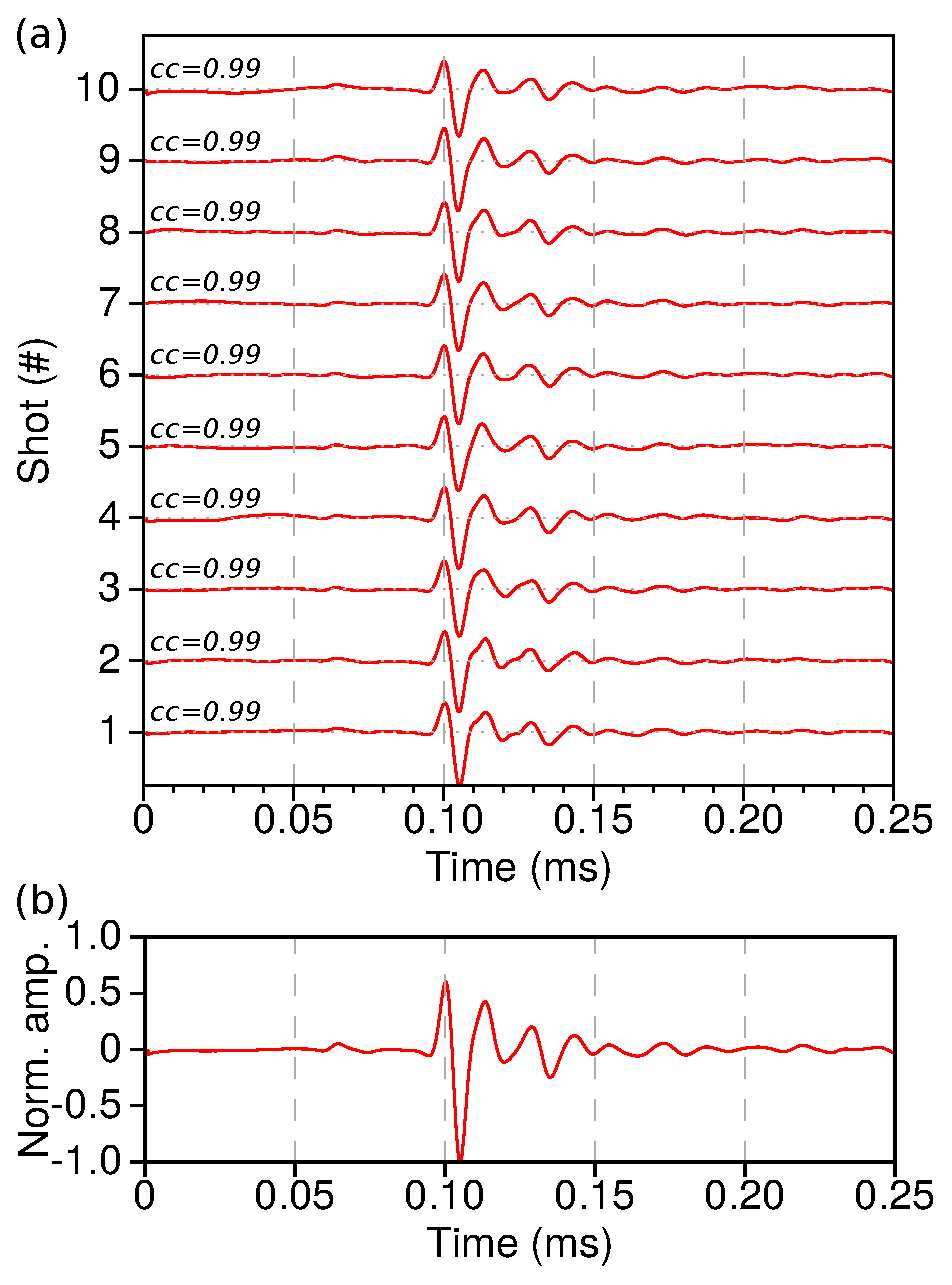
\includegraphics[scale=1.0]{fig/musc_F50_CT.eps}
	\caption{Central trace for each of the ten analogic experiment. \textbf{cc} gives the correlation factor of each central trace with respect to a mean trace.}
	\label{panel_srcest_2d_mean}
\end{figure}

\begin{figure}[!h]
	\centering
	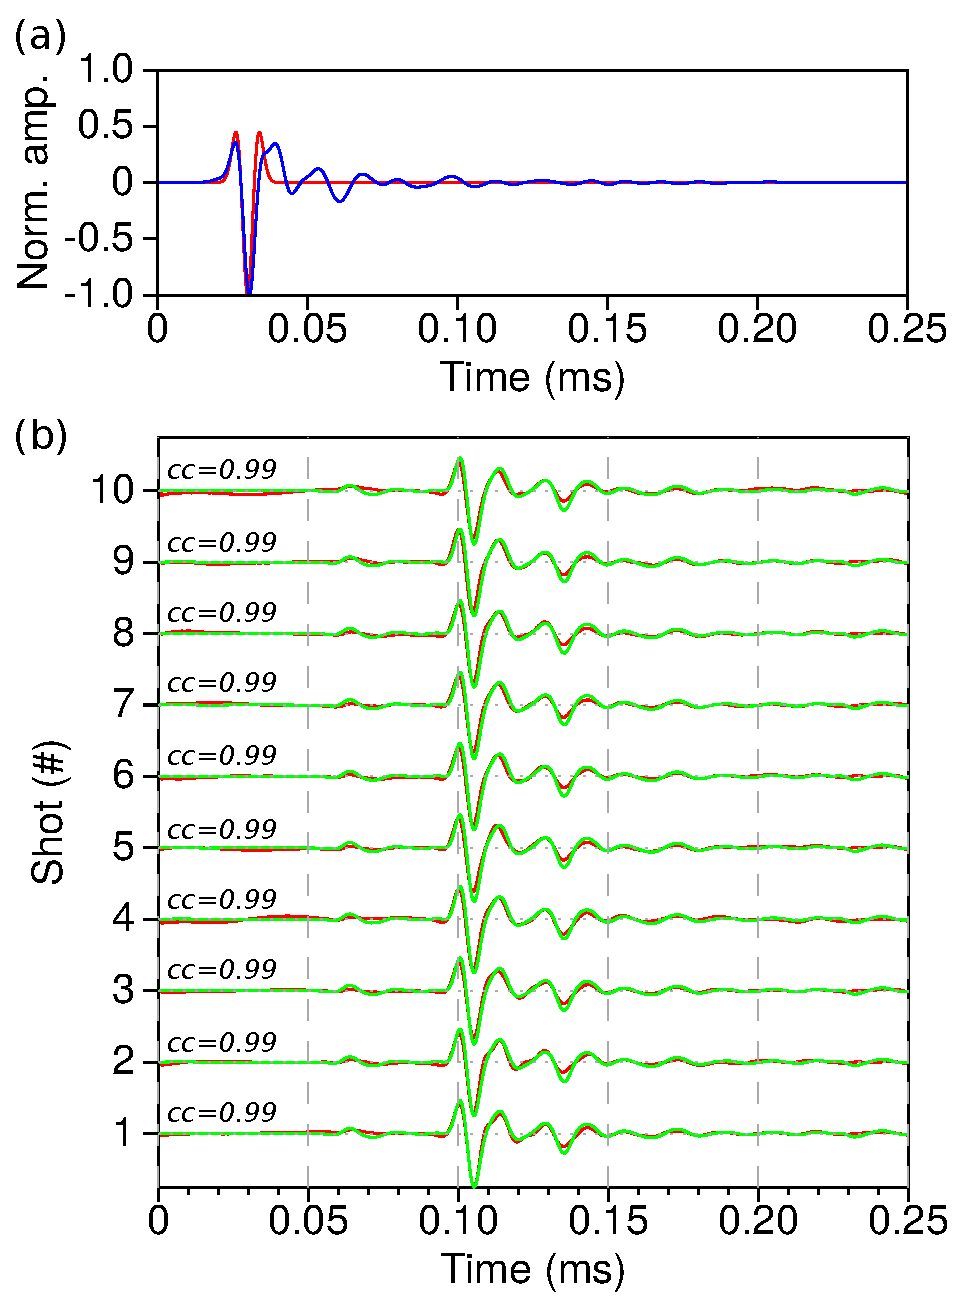
\includegraphics[scale=1.0]{fig/spec_F50_CT_COMP.eps}
	\caption{Comparison between analogic central traces (grey) and numerical traces corrected from the estimated effective source (black) for each experiment. \textbf{cc} gives the correlation coefficient.}
	\label{panel_srcest_2d_mean_comp}
\end{figure}

\clearpage
\newpage

\subsection*{Tables}

\begin{table}[!ht]
	\centering
	\begin{tabular}{cccccc}
		\hline
		material & $\mathrm{V_{P}\ (m/s)}$ & $\mathrm{V_{S}\ (m/s)}$ & $\mathrm{V_{R}\ (m/s)}$ & $\mathrm{\rho\ (kg/m^{3})}$ & $\mathrm{Q}$ \\
		\hline
		Aluminium & 5630 & 3225 & --   & 2700 & --  \\
		F50 pure  & 2300 & 1030 & 965  & 1300 & 30  \\
		F50 200\% & 2820 & 1425 & 1328 & 1766 & --  \\
		F50 240\% & 2968 & 1496 & 1388 & 1822 & --  \\
		LAB1000   & 2850 & 1400 & 1310 & 1500 & 75  \\
		\hline
	\end{tabular}
	\caption{Physical properties of some materials used to build small scale models. $\mathrm{V_{P}}$, $\mathrm{V_{S}}$ and $\mathrm{V_{R}}$ are the P-wave velocity, S-wave and the Rayleigh wave velocity, respectively. $\rho$ is the density and $\mathrm{Q}$ is the quality factor.}
	\label{epoxy-resin}
\end{table}

\clearpage
\newpage

\begin{table}[!ht]
	\centering
	\begin{tabular}{lcccc}
		\hline
		\qquad & 90 mm & 95 mm & 100 mm & 105 mm \\
		\hline
		$cc1_{init}$  & 0.702 & 0.725 & 0.728 & 0.728 \\
		$rms1_{init}$ & 0.794 & 0.760 & 0.762 & 0.774 \\
		\hline
		$cc1_{final}$  & 0.940 & 0.953 & 0.951 & 0.949 \\
		$rms1_{final}$ & 0.358 & 0.317 & 0.325 & 0.343 \\
		\hline
		\hline
		$cc2_{init}$  & 0.954 & 0.987 & 0.988 & 0.988 \\
		$rms2_{init}$ & 0.304 & 0.162 & 0.155 & 0.154 \\
		\hline
		$cc2_{final}$  & --   & --    & --    & --    \\
		$rms2_{final}$ & --   & --    & --    & --    \\
		\hline
	\end{tabular}
	\caption{.}
	\label{cc-rms}
\end{table}

\clearpage
\newpage 

\section{ACKNOWLEDGMENTS}

\clearpage
\newpage

\bibliographystyle{seg}  % style file is seg.bst
%\bibliography{/media/pageotd/1581-58C8/Work/git-repository//TR-VIBRIS/tail/bibvibris}
\bibliography{../TR-VIBRIS/tail/bibvibris}

\end{document}
